\documentclass[../main.tex]{subfiles}

\begin{document}

\ifSubfilesClassLoaded{

    %\tableofcontents
    
    %\setcounter{chapter}{}
}{}

\chapter{ Medium Test 2023 }
% 代靖涵 25120222201319
\begin{exercise}{}{}
\begin{enumerate}
    \item 设 $A, B, C$ 为三个随机事件, 试叙述 “\dfntxt{A, B, C 相互独立}” 的定义;
    \item 有一均匀的正四面体, 其中三个面分别染成了红, 黄, 蓝三种颜色, 剩下的一个面染成了彩色(红, 黄, 蓝各占一部分). 现在桌上将此四面体随意掷出, 考察与桌面相接触的那一面上出现的颜色. 记 $A = $ 红色出现, $B = $ 黄色出现, $C = $ 蓝色出现. 试判断 $A, B$ 和 $C$ 的独立性.
\end{enumerate}
\end{exercise}

\begin{proof}
    \begin{enumerate}
        \item 称 \(  A,B,C  \)相互独立, 若 \[
        P\left( AB \right)= P\left( A \right)P\left( B \right) ,\quad P\left( AC \right)= P\left( A \right)P\left( C \right),\quad P\left( BC \right)= P\left( B \right)P\left( C \right)         
        \]且 \[
        P\left( ABC \right)= P\left( A \right)P\left( B \right)P\left( C \right)    
        \] 
        \item  \[
        P\left( A \right)= P\left( B \right)= P\left( C \right)= \frac{1 }{2 }    
        \] \[
        P\left( AB \right)= P\left( BC \right)= P\left( AC \right)= P\left( ABC \right)= \frac{1 }{4 }     
        \]我们有\[
        P\left( AB \right)= P\left( A \right)P\left( B \right) = P\left( AC \right)= P\left( A \right)P\left( C \right)=  P\left( BC \right)= P\left( B \right)P\left( C \right)   =       \frac{1 }{4 } 
        \] \[
        P\left( ABC \right)\neq P\left( A \right)P\left( B \right)P\left( C \right)    
        \]因此 \(  A,B,C  \)两两独立但不是相互独立的. 
    \end{enumerate}
    
\end{proof}
\begin{exercise}{}{}
\begin{enumerate}
    \item 设 $X$ 服从几何分布, 试证明 $X$ 具有无记忆性, 即对任意正整数 $m$ 和 $n$ 都有 $P(X > m+n | X > m) = P(X > n)$ 成立;
    \item 设 $X$ 是取正整数值的离散型随机变量. 试证若 $X$ 满足无记忆性, 则 $X$ 必然服从几何分布.
\end{enumerate}
\end{exercise}
\begin{proof}
    \begin{enumerate}
        \item \[
        P\left( X= k \right)= \left( 1-p \right)^{k-1}p  
        \]对于任意的正整数 \(  m  \), 由于 \(  \left( 1-p \right)< 1   \), 我们有   \[
        P\left( X> m \right)= \sum _{k= m+ 1}^{\infty}\left( 1-p \right)^{k-1}p=   \left( 1-p \right)^{m}\frac{1 }{1-\left( 1-p \right)  }p= \left( 1-p \right)^{m} 
        \]我们有 \[
        \begin{aligned}
        P\left( X> m+ n|X> m \right)&=  \frac{P\left( \left\{ X> m+ n \right\}\cap \left\{ X> m \right\} \right)  }{P\left( X> m \right)  }   \\ 
         &= \frac{P\left( X> m+ n \right)  }{P\left( X> m \right)  }\\ 
          &=\frac{\left( 1-p \right)^{m+ n}  }{\left( 1-p \right)^{m}  } 
           &=   \left( 1-p \right)^{n}\\ 
            &= P\left( X> n \right)  
        \end{aligned}
        \]

        \item 若 \(  X  \)满足无记忆性, 则  \[
        P\left( X> m+ 1| X> m \right)= P\left( X> 1 \right)  
        \]其中 \[
        P\left( X> m+ 1|X> m \right)= \frac{P\left( \left\{ X> m+ 1 \right\}\cap \left\{ X> m \right\} \right)  }{P\left( X> m \right)  }= \frac{P\left( X> m+ 1 \right)  }{P\left( X> m \right)  }   
        \]于是 \[
        P\left( X> m+ 1 \right)= P\left( X> m \right)P\left( X> 1 \right)   
        \] 令 \(  P\left( X= 1 \right)= p   \) , 则 \[
        P\left( X> m+ 1 \right)= P\left( X> m \right)\left( 1-p \right)   
        \]进而 \[
        \left( 1-P\left( X\le m+ 1 \right)  \right)= \left( 1-P\left( X\le m \right)  \right)\left( 1-p \right)   
        \]得到 \[
        P\left( X\le m+ 1 \right)= \left( 1-p \right)P\left( X\le m \right)+ p   
        \] 设 \(  F  \)是 \(  X  \)的累积分布函数, 则 \[
        F\left( m+ 1 \right)= \left( 1-p \right)F\left( m \right)+ p   
        \]   \[
        F\left( m+ 1 \right)-1 = \left( 1-p \right)\left( F\left( m \right)-1  \right)  
        \]从而 \[
        F\left( m \right)-1= \left( 1-p \right)^{m-1}\left( F\left( 1 \right)-1  \right)= \left( 1-p \right)^{m-1}\left( p-1 \right)     
        \] \[
        F\left( m \right)= 1-\left( 1-p \right)^{m}  = \sum _{k= 1}^{m}\left( 1-p \right)^{k-1}p 
        \]这表明 \(  X  \)服从参数为\(  p  \)的几何分布.  
    \end{enumerate}
    
\end{proof}
\begin{exercise}{}{}
设 $\varphi(x)$ 是标准正态分布的密度函数:
\begin{enumerate}
    \item 求证 $\varphi(x)$ 满足方程 $\varphi'(x) + x\varphi(x) = 0$;
    \item 求证当 $x > 0$ 时有不等式
    $$\begin{aligned}
    \left(\frac{1}{x} - \frac{1}{x^3}\right)\varphi(x) < 1 - \Phi(x) < \left(\frac{1}{x} - \frac{1}{x^3} + \frac{3}{x^5}\right)\varphi(x)
    \end{aligned}$$
    成立, 其中 $\Phi(x)$ 是标准正态分布的分布函数.
\end{enumerate}
\end{exercise}
\begin{proof}
    \begin{enumerate}
        \item  \[
         \varphi \left( x \right)= \frac{1 }{\sqrt{2 \pi } }e^{-\frac{x^{2} }{2 } }  
        \] \[
         \varphi ^{\prime} \left( x \right)= \frac{1 }{\sqrt{2 \pi } }\left( -xe^{-\frac{x^{2} }{2 } } \right)= -x  \varphi \left( x \right)    
        \]故 \[
         \varphi ^{\prime} \left( x \right)+ x \varphi \left( x \right)= 0  
        \]
        \item 对于 \(  x> 0  \),  \[
        \frac{ \varphi ^{\prime} \left( x \right)  }{x }+  \varphi \left( x \right)= 0  
        \] 两边从\(  x  \)到 \(  \infty  \)积分, 得到  \[
        \int_{x}^{\infty}\frac{ \varphi ^{\prime} \left( x \right)  }{x }\,\mathrm{d} x+ 1- \Phi \left( x \right)= 0  
        \]其中 \[
        \begin{aligned}
        \int_{x}^{\infty}\frac{ \varphi ^{\prime} \left( x \right)  }{x }\,\mathrm{d} x&= \int_{x}^{\infty}\frac{1 }{x }\,\mathrm{d}  \varphi \left( x \right)\\ 
         &=- \frac{ \varphi \left( x \right)  }{x }+ \int_{x}^{\infty}  \varphi \left( x \right)\,\mathrm{d} \frac{1 }{x }\\ 
          &=- \frac{ \varphi \left( x \right)  }{x }+ \int_{x}^{\infty} \frac{1 }{x^{2} }\varphi \left( x \right)\,\mathrm{d} x          \\ 
           &=- \frac{ \varphi \left( x \right)  }{x }- \int_{x}^{\infty} \frac{ \varphi ^{\prime} \left( x \right)  }{x^{3} }\,\mathrm{d} x\\ 
            &= -\frac{ \varphi \left( x \right)  }{x }+  \frac{ \varphi \left( x \right)  }{x^{3} }-3\int_{x}^{\infty}\frac{1 }{x^{4} } \varphi \left( x \right)\,\mathrm{d} x  \le  \varphi \left( x \right)\left( -\frac{1 }{x }+ \frac{1 }{x^{3} }   \right)     \\ 
             &= -\frac{ \varphi \left( x \right)  }{x }+ \frac{ \varphi \left( x \right)  }{x^{3} }+ 3\int_{x}^{\infty}\frac{1 }{x^{5} } \varphi ^{\prime} \left( x \right)\,\mathrm{d} x\\ 
              &= - \varphi \left( x \right)     \left( \frac{1 }{x }-\frac{1 }{x^{3} }+ \frac{3 }{x^{5} }    \right) + 15\int_{x}^{\infty}\frac{1 }{x^{6} } \varphi \left( x \right)\,\mathrm{d} x\ge - \varphi \left( x \right)\left( \frac{1 }{x }-\frac{1 }{x^{3} }+ \frac{3 }{x^{5} }    \right)    
        \end{aligned}
        \]其中第四行和第六行使用了微分方程, 将第五行和第七行中的不等式带入回积分方程, 即可得到题述的两个不等式.
    \end{enumerate}
    
\end{proof}
\begin{exercise}{单边 Chebyshev 不等式}{}
设随机变量 $X$ 的方差存在, 记为 $\operatorname{Var}(X) = \sigma^2$, 求证对任意 $x > 0$ 和 $a > 0$, 有如下不等式成立:
$$\begin{aligned}
P\{X - E(X) \ge x\} \le \frac{a^2 + \sigma^2}{(x+a)^2}
\end{aligned}$$
\end{exercise}
\begin{proof}
      \[
 \begin{aligned}
 \left( x+ a \right)^{2}  P\left\{ X-E\left( X \right)\ge x  \right\}&=  \int \chi _{\left\{ X-\mu \ge x \right\}}\left( x^{2}+ 2ax+ a^{2} \right)   \,\mathrm{d} P\\ 
  &\le  \int \chi _{\left\{ X-\mu \ge x \right\}}\left( \left( X-\mu  \right)^{2}+ 2a\left( X-\mu  \right)+ a^{2}   \right) \,\mathrm{d} P \\ 
   &\le  \int \left( X-\mu + a \right)^{2}\mathrm{d} P\\ 
    &= E\left( \left( X-\mu  + a\right)^{2}  \right)=  \sigma ^{2}+2aE\left( X-\mu  \right)+ a^{2} \\ 
     &=  \sigma ^{2}+ a^{2}
 \end{aligned}
      \]故 \[
      P\left\{ X-E\left( X \right)\ge x  \right\}\le \frac{a^{2}+  \sigma ^{2} }{\left( x+ a \right)^{2}  } 
      \]
\end{proof}
\begin{exercise}{}{}
从 5 双不同鞋子中任取 4 只, 4 只鞋子中至少有 2 只配成一双的概率是多少.
\end{exercise}
\begin{solution}
   无双不同鞋子取\(  4  \)只的取法共有 \(  C_{10}^{4}  \)中, 4只鞋子中仅配成一对的情况有 \( C_{5}^{1}\times C_{4}^{2}\times C_{2}^{1}\times C_{2}^{1}   \) 种, 配成两双的情况有 \(  C_{5}^{2}  \)中 , 于是概率为   \[
    \frac{ C_{5}^{1}C_{4}^{2}C_{2}^{1}C_{2}^{1}+ C_{5}^{2}}{C_{10}^{4} } = \frac{120+ 10 }{210 }= \frac{13 }{21 }  
    \] 
\end{solution}

\begin{exercise}{}{}
设有 4 个独立工作的元件 1, 2, 3, 4. 它们的可靠性分别为 $P_1, P_2, P_3, P_4$, 将他们按下图的方式联接, 求系统的可靠性概率.
\begin{center}
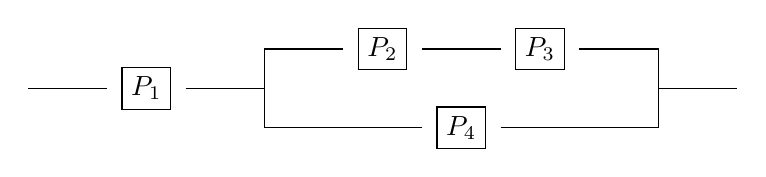
\begin{tikzpicture}
    \draw (0,0) -- (1,0);
    \node[draw, rectangle] at (1.5,0) {$P_1$};
    \draw (2,0) -- (3,0);
    
    \draw (3,0) -- (3,0.5) -- (4,0.5);
    \node[draw, rectangle] at (4.5,0.5) {$P_2$};
    \draw (5,0.5) -- (6,0.5);
    \node[draw, rectangle] at (6.5,0.5) {$P_3$};
    \draw (7,0.5) -- (8,0.5) -- (8,0);

    \draw (3,0) -- (3,-0.5) -- (5,-0.5);
    \node[draw, rectangle] at (5.5,-0.5) {$P_4$};
    \draw (6,-0.5) -- (8,-0.5) -- (8,0);

    \draw (8,0) -- (9,0);
\end{tikzpicture}
\end{center}
\end{exercise}

\begin{solution}
    设 \(  A_{i}  \)为第 \(  i  \)个原件可靠的事件, \(  i= 1,2,3,4  \)  则 \(P\left( A_{i} \right)= P_{i}    \).   系统是可靠的概率为 \[
    P\left( A_1\cap \left( \left( A_2\cap A_3 \right)\cup A_4  \right)  \right) 
    \]由于原件是独立的, 我们有 \[
    P\left( A_1\cap \left( \left( A_2\cap A_3 \right)\cup A_4  \right)  \right)= P\left( A_1 \right)  P\left( \left( A_2\cap A_3 \right)\cup A_4  \right) 
    \]其中 \[
   \begin{aligned}
    P\left( \left( A_2\cap A_3 \right)\cup A_4  \right)&= P\left( A_2\cap A_3 \right)+ P\left( A_4 \right)-P\left( \left( A_2\cap A_3 \right)\cap A_4  \right)     \\ 
     &= P\left( A_2 \right)P\left( A_3 \right)+ P\left( A_4 \right)-P\left( A_2 \right)P\left( A_3 \right)P\left( A_4 \right)\\ 
      &= P_2P_3+ P_4-P_2P_3P_4      
   \end{aligned}
    \]于是 \[
    P\left( A_1\cap \left( \left( A_2\cap A_3 \right)\cup A_4  \right)  \right)= P_1\left( P_2P_3+ P_4-P_2P_3P_4 \right)  
    \]
\end{solution}

\begin{exercise}{}{}
将 $A, B, C$ 三个字母之一输入信道, 输出为原字母的概率为 $a$, 而输出为其它二字母的概率都是 $(1-a)/2$. 今将字母串 AAAA, BBBB, CCCC 之一输入信道, 输入 AAAA, BBBB, CCCC 的概率分别为 $p_1, p_2, p_3$ ($p_1 + p_2 + p_3 = 1$), 已知输出为 ABCA, 问输入的是 AAAA 的概率是多少? (设信道传输每个字母的工作是相互独立的)
\end{exercise}

\begin{solution}
设 \(  A_0, B_0,C_0  \)分别为输如 \(  AA A A, B  B B B, C C C C  \)的事件.
 \[
 \begin{aligned}
 P\left( A_0| A B C A\right)&= \frac{P\left( A B C A \cap A_0 \right)  }{P\left( A B C A\right)  }\\ 
  &=    \frac{P\left( AB C A|A_0\right)P\left( A_0 \right)   }{P\left( A B C A |A_0 \right)P\left( A_0 \right)+ P\left( A B C A|B_0 \right)P\left( B_0 \right)+ P \left( A B C A|C_0 \right)P\left( C_0 \right)       } 
 \end{aligned}
 \] 其中 \[
 P\left( A B C A|A_0 \right)= \frac{1 }{2^{2} }a^{2}\left( 1-a \right)^{2}   
 \] \[
 P\left( ABCA|B_0 \right)= \frac{1   }{2^{3}}a\left( 1-a \right)^{3}   
 \] \[
 P\left( ABCA |C_0 \right)= \frac{1 }{2^{3} } a \left( 1-a \right)^{3}   
 \]于是 \[
 \begin{aligned}
 P\left( A_0|ABCA \right)&= \frac{\frac{1 }{2^{2} }a^{2}\left( 1-a \right)^{2}p_1   }{ \frac{1 }{2^{2} }a^{2}\left( 1-a \right)^{2}p_1+ \frac{1 }{2^{3} }a\left( 1-a \right)^{3}p_2+ \frac{1 }{2^{3} }a\left( 1-a \right)^{3}p_3      }  \\ 
  &= \frac{2ap_1  }{2ap_1+ \left( 1-a \right)\left( p_2+ p_3 \right)   }\\ 
   &=  \frac{2ap_1 }{2ap_1+ \left( 1-a \right)\left( 1-p_1 \right)   }\\ 
    &= \frac{2ap_1 }{\left( 3a-1 \right)p_1+ \left( 1-a \right)   }  
 \end{aligned} 
 \]为输入的是 AAAA的概率.
\end{solution}

\end{document}